\subsection*{SyntaxSQLNet}
% [2] Yu, Tao, et al. “Syntaxsqlnet: Syntax tree networks for the complex and cross-domain text-to-SQL task.” arXiv preprint arXiv:1810.05237 (2018).

\begin{itemize}
    \item The main goal of developing the SyntaxSQLNet model was to generate complex SQL queries with multiple clauses and generalize them to new databases.
    \item The model is based on a syntax tree network to address complex and cross-domain queries. The encoders are table-aware, and the decoders have a history of the SQL generation path.
    \item With a massive 7.3\% improvement in accuracy, SyntaxSQLNet outperformed previous models, such as SQLNet, on the SPIDER dataset.
\end{itemize}


\begin{figure}[htb]
    \centering
    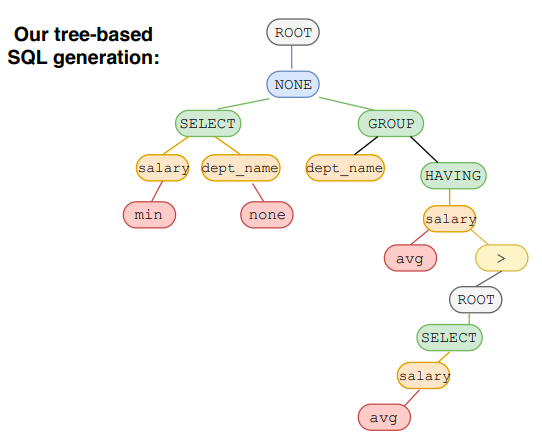
\includegraphics[width=0.8\textwidth]{pics/SyntaxSQLNet/Tree-based.png}
    \caption{Tree-based SQL generator in SyntaxSQLNet}
    \label{fig:tree-based}
\end{figure}

\begin{itemize}
    \item A cross-domain data augmentation technique further improves accuracy by generating more variance during training.
    \item Below is a chart showing the various modules and their functions.
\end{itemize}

\begin{figure}[htb]
    \centering
    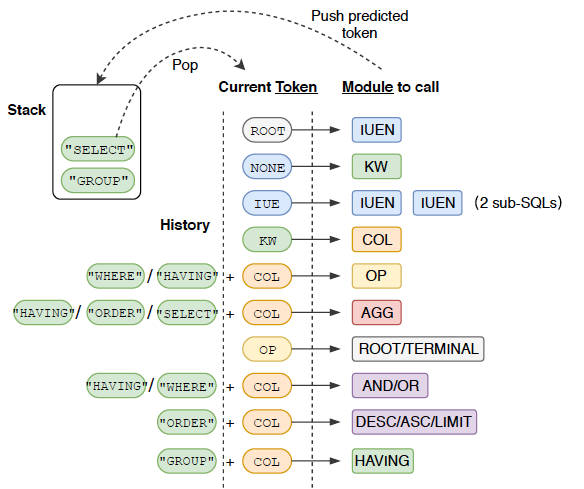
\includegraphics[width=0.8\textwidth]{pics/SyntaxSQLNet/Grammar.png}
    \caption{Modules defined in SyntaxSQLNet model}
    \label{fig:grammar}
\end{figure}


\textbf{SQL Grammar and Attention Mechanism}

\begin{itemize}
    \item In order to enable the decoder to handle complex queries, SQL grammar is used. At each step of recursive decoding, it determines which module to invoke.
    \item Predicting the next SQL token is also based on the history of SQL path generation and current SQL tokens.
    \item The attention mechanism is also used to encode the question representation. Attention also applies to SQL path history encoding.
\end{itemize}

\begin{figure}[htb]
    \centering
    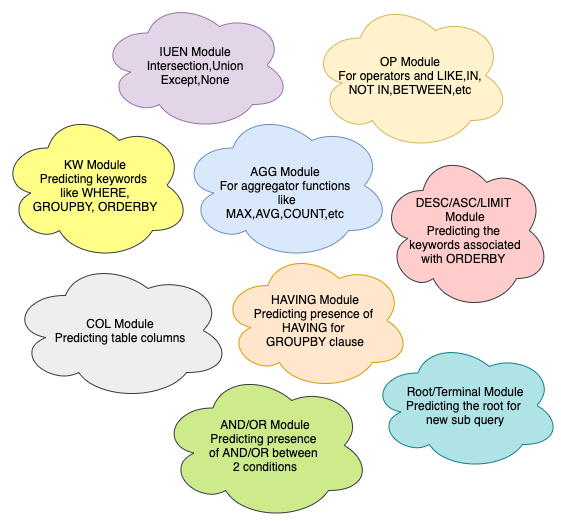
\includegraphics[width=0.8\textwidth]{pics/SyntaxSQLNet/Modules.png}
    \caption{Modules and SQL Grammar used in the decoding process}
    \label{fig:modules}
\end{figure}


\textbf{Data Augmentation}

\begin{itemize}
    \item Despite SPIDER's large dataset, it lacks complex queries.
    \item For proper generalization, cross-domain datasets are used for data augmentation.
    \item Various training databases of the SPIDER dataset are used to prepare a list of patterns for natural language questions and corresponding SQL queries.
\end{itemize}

The SPIDER model using syntaxSQLNet decoding history reaches 27.2\% accuracy.


Compared to previous models, such as SQLNet, the accuracy increased by 15\%.